\documentclass[11pt,a4paper]{article}

\usepackage[margin=1in]{geometry}
\usepackage{amsmath}
\usepackage{graphicx}
\usepackage[T1]{fontenc}
\usepackage[utf8]{inputenc}
\usepackage{lmodern}
\usepackage[hidelinks]{hyperref}

\graphicspath{{docs/images/algorithms/}{../images/algorithms/}}

\title{FFT Amplitude and Welch PSD\\A Small Algorithm Note}
\author{EvalData Repository Example}
\date{April 2026}

\begin{document}

\maketitle

\section{Purpose}

This document is a small LaTeX example for the repository. It explains two frequency-analysis methods used in the app: FFT amplitude and Welch power spectral density (PSD).

The goal is not to be mathematically exhaustive. The goal is to show the kind of formal algorithm note that fits well in LaTeX: what the method is for, the basic principle, where it works well, and where users should be careful.

\section{When to Use Each Method}

\subsection{FFT Amplitude}

Use FFT amplitude when you want a direct view of the dominant periodic content of a signal.

Typical use cases:

\begin{itemize}
    \item checking whether a clean signal contains one or a few strong frequencies,
    \item locating dominant peaks quickly,
    \item comparing how spectral peaks move between datasets.
\end{itemize}

\subsection{Welch PSD}

Use Welch PSD when the signal is noisy, long, or statistically variable and you want a smoother spectral estimate.

Typical use cases:

\begin{itemize}
    \item estimating the frequency distribution of noisy signals,
    \item reducing variance in the spectrum estimate,
    \item comparing broadband energy trends instead of only sharp peaks.
\end{itemize}

\section{FFT Amplitude Principle}

For a discrete signal $x[n]$ of length $N$, the discrete Fourier transform is

\[
X[k] = \sum_{n=0}^{N-1} x[n] e^{-j 2 \pi kn / N}.
\]

The amplitude spectrum is built from $|X[k]|$, usually after mapping the frequency bins to physical frequency using the sample spacing.

In practical terms, the FFT converts a time-domain or index-domain signal into a frequency-domain representation and answers the question: \emph{which frequencies are present, and how strong are they?}

\subsection{Strengths}

\begin{itemize}
    \item direct and easy to interpret for clean periodic signals,
    \item computationally efficient,
    \item very good for locating dominant spectral peaks.
\end{itemize}

\begin{figure}[h]
    \centering
    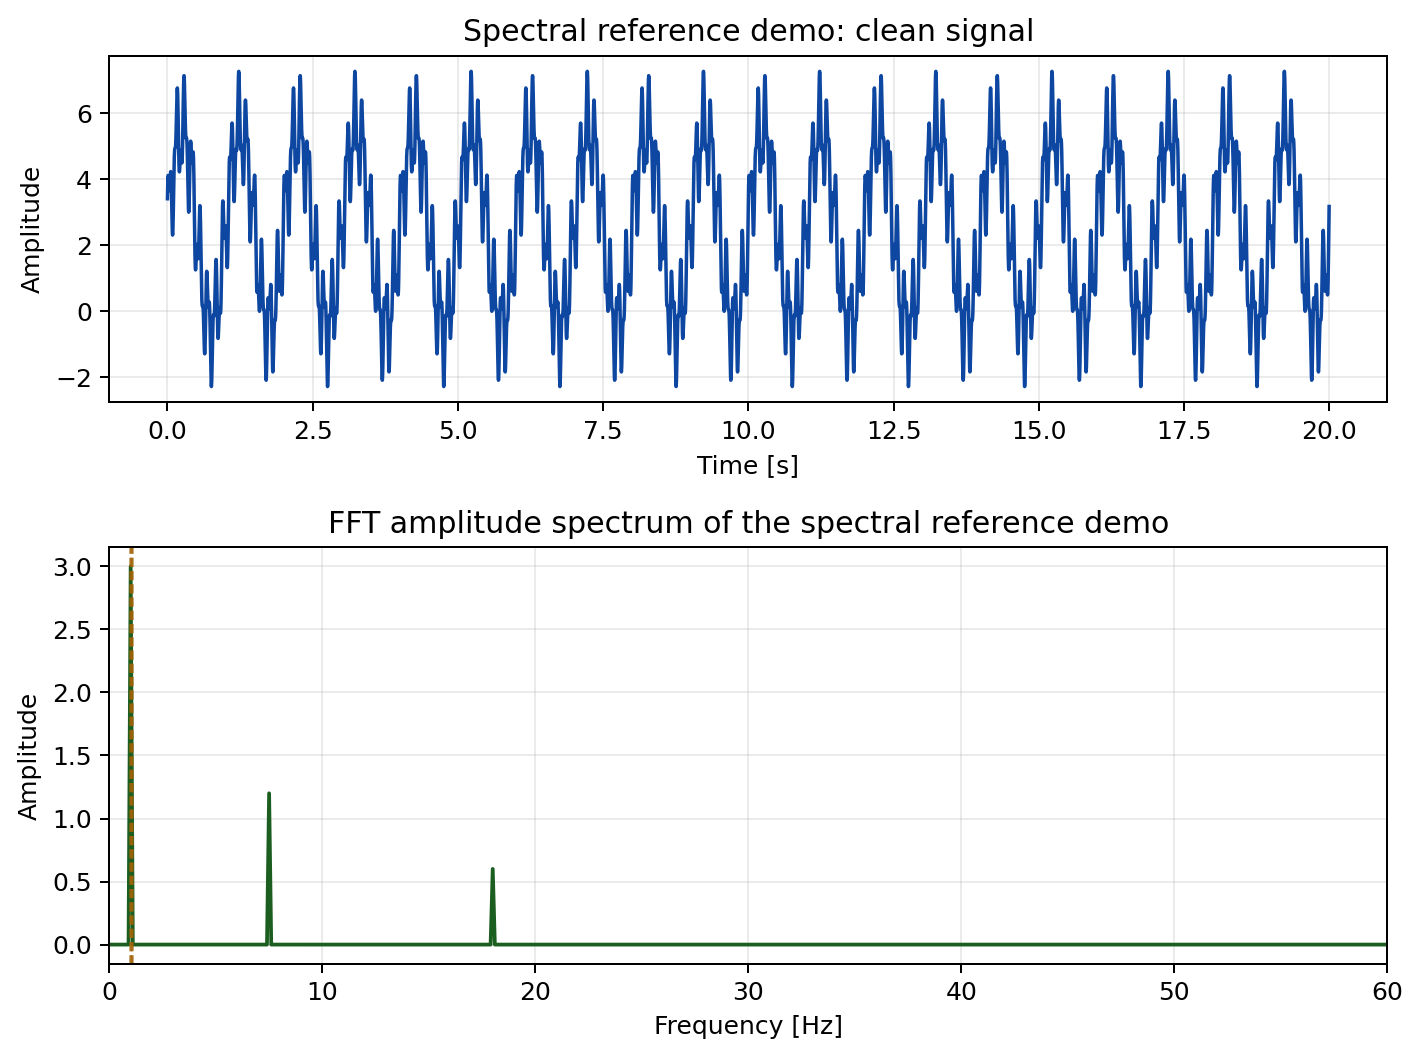
\includegraphics[width=0.9\linewidth]{fft_clean_signal.png}
    \caption{The built-in spectral reference demo and its FFT amplitude spectrum. This is the kind of case where dominant peaks are easy to locate directly.}
\end{figure}

\subsection{Caveats}

\begin{itemize}
    \item The result depends strongly on sample spacing and the meaning of the x-axis.
    \item Finite data windows cause spectral leakage when the signal does not align well with the observation window.
    \item Window choice and detrending matter.
    \item Amplitude spectra from different preprocessing choices are not always directly comparable.
\end{itemize}

\section{Welch PSD Principle}

Welch's method estimates power spectral density by splitting the signal into overlapping segments, windowing each segment, computing a periodogram for each one, and averaging the results.

In simplified form,

\[
\hat{S}_{xx}(f) = \frac{1}{L} \sum_{\ell=1}^{L} P_{\ell}(f),
\]

where $P_{\ell}(f)$ is the periodogram of segment $\ell$ and $L$ is the number of segments.

In practical terms, Welch PSD answers the question: \emph{how is signal power distributed across frequency, with reduced estimate variance compared to a single full-length FFT?}

\subsection{Strengths}

\begin{itemize}
    \item smoother and more stable than a single raw spectrum estimate,
    \item useful for noisy measurements,
    \item often better for seeing broadband trends.
\end{itemize}

\begin{figure}[h]
    \centering
    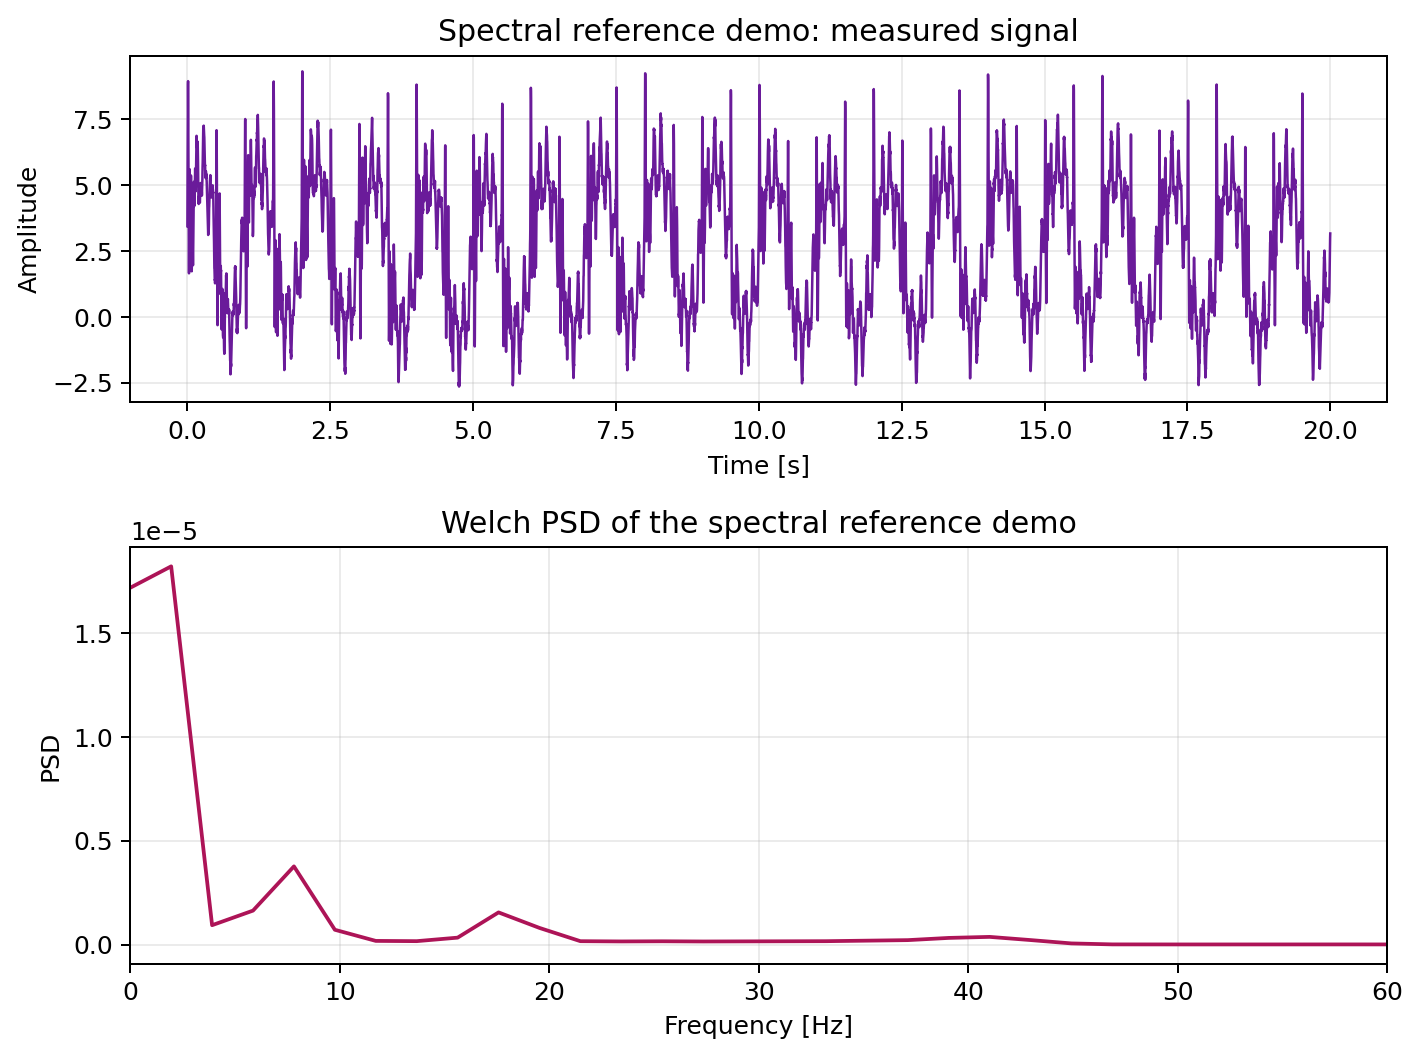
\includegraphics[width=0.9\linewidth]{welch_noisy_signal.png}
    \caption{The measured channel from the built-in spectral reference demo and its Welch PSD estimate. Averaging across segments produces a smoother spectral view.}
\end{figure}

\subsection{Caveats}

\begin{itemize}
    \item Smoothing reduces variance but also reduces frequency resolution.
    \item Segment length and overlap strongly affect the result.
    \item Welch PSD is a power estimate, not the same thing as a direct amplitude spectrum.
    \item Users can misread PSD peaks as if they were identical to FFT peak magnitudes.
\end{itemize}

\section{FFT Amplitude vs. Welch PSD}

\begin{figure}[h]
    \centering
    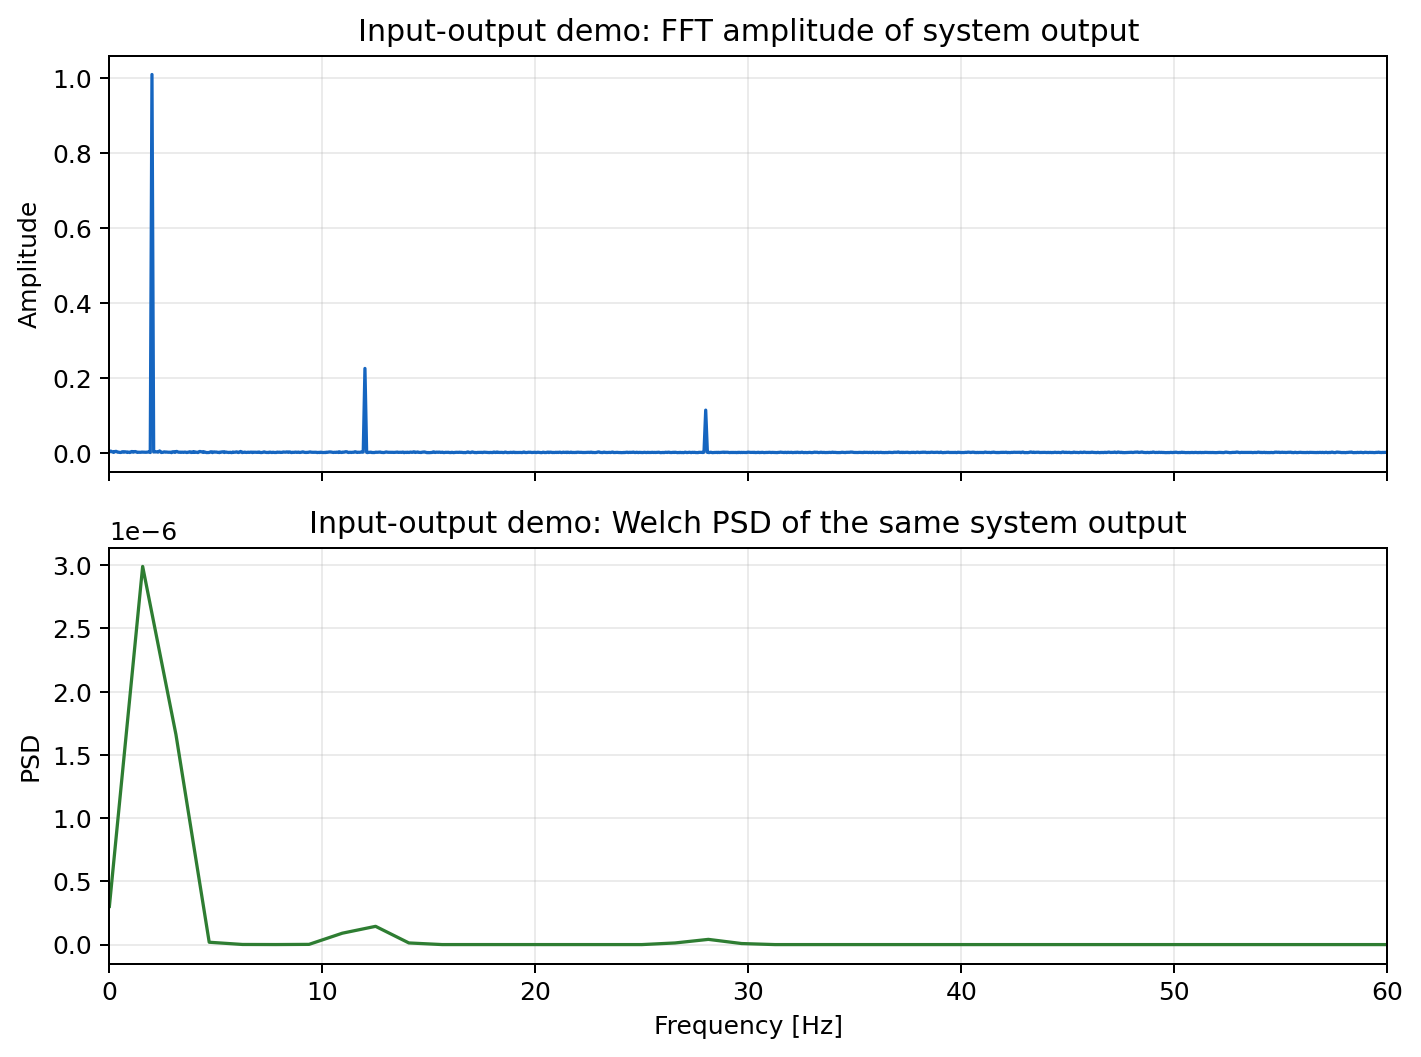
\includegraphics[width=0.9\linewidth]{fft_vs_welch_comparison.png}
    \caption{FFT amplitude and Welch PSD applied to the built-in input-output demo system output. The FFT is sharper, while Welch PSD is smoother and less variable.}
\end{figure}

\begin{center}
\begin{tabular}{|p{0.18\linewidth}|p{0.31\linewidth}|p{0.31\linewidth}|}
\hline
Aspect & FFT Amplitude & Welch PSD \\
\hline
Main goal & Find strong frequencies & Estimate spectral power more smoothly \\
\hline
Best for & Clean periodic content & Noisy or broadband signals \\
\hline
Resolution & Higher for full record & Lower because of segment averaging \\
\hline
Variance & Higher & Lower \\
\hline
Interpretation risk & Leakage and scaling confusion & PSD vs amplitude confusion \\
\hline
\end{tabular}
\end{center}

\section{Use in EvalData}

In EvalData, these methods are most useful after the user has already:

\begin{itemize}
    \item selected the right dataset,
    \item assigned the correct time or reference column,
    \item chosen the right active signal,
    \item trimmed the dataset to the relevant output range if needed.
\end{itemize}

That is important because many apparent algorithm problems are actually setup problems: wrong axis interpretation, wrong signal column, or data ranges that contain non-stationary sections.

\begin{figure}[h]
    \centering
    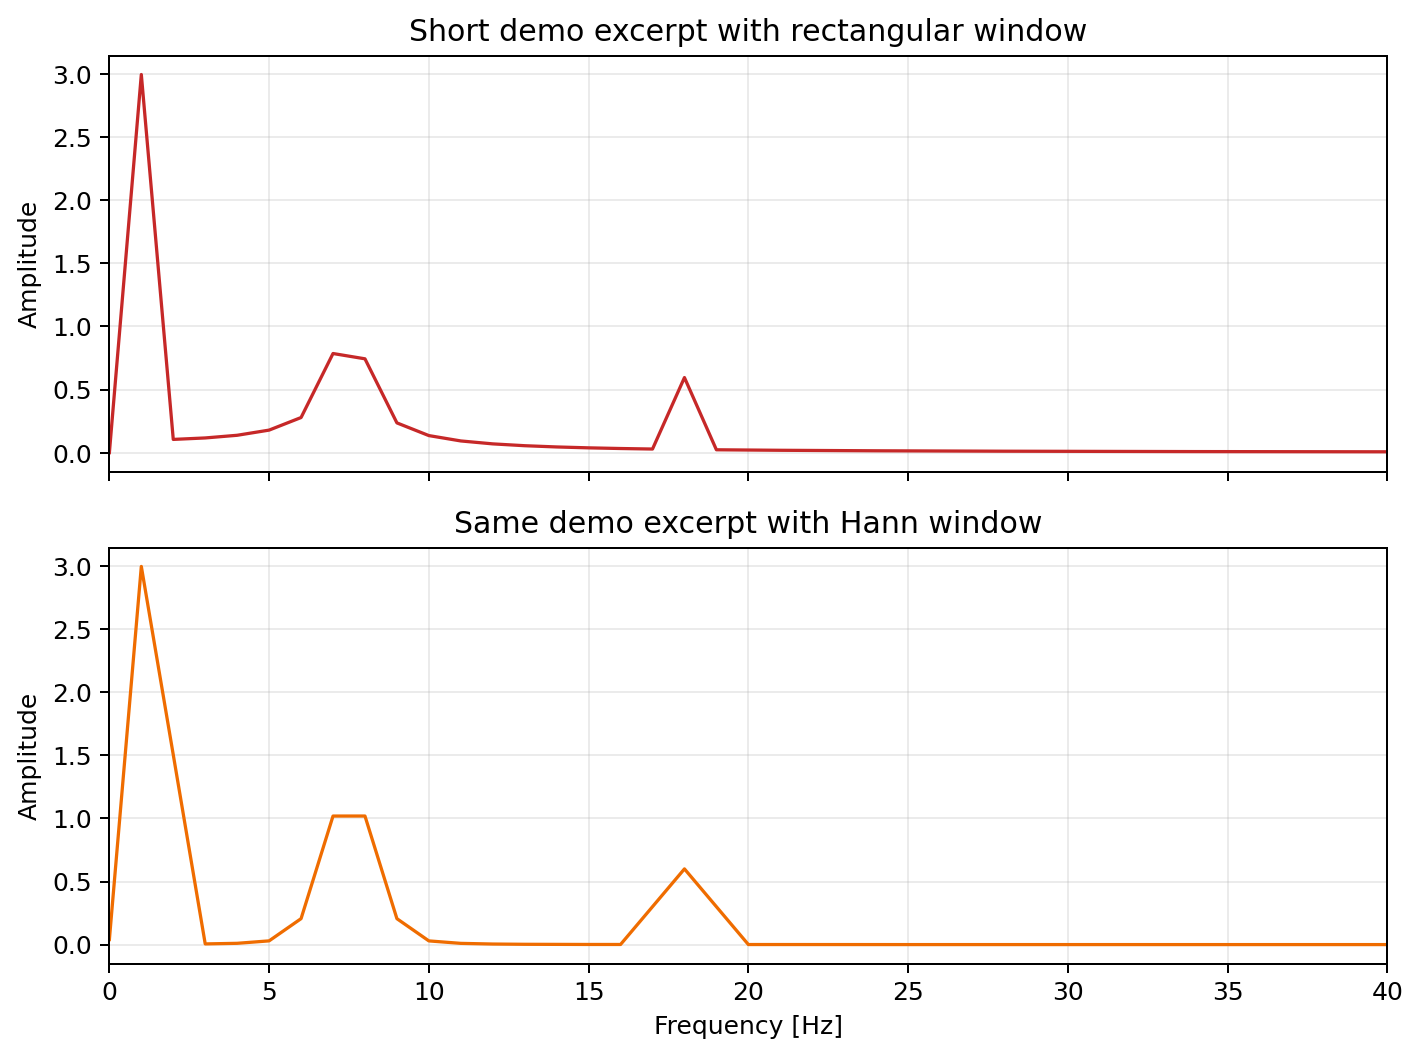
\includegraphics[width=0.9\linewidth]{window_leakage_comparison.png}
    \caption{Leakage-style comparison using a short excerpt of the built-in spectral reference demo. Window choice changes how energy spreads across nearby frequencies when the observation window is short.}
\end{figure}

\section{Practical Guidance}

Use FFT amplitude first when you want a fast answer to ``what peaks are present?''

Use Welch PSD when the FFT looks too noisy or when you care more about stable power distribution than exact peak height.

If both methods tell a different story, do not assume one is wrong immediately. First check:

\begin{itemize}
    \item sample spacing,
    \item signal length,
    \item window settings,
    \item detrending choice,
    \item whether the data segment is stationary enough for spectral interpretation.
\end{itemize}

\section{Conclusion}

FFT amplitude and Welch PSD are complementary rather than interchangeable. FFT amplitude is often the clearest first inspection tool. Welch PSD is often the more stable estimate for noisy real-world data. Good documentation should explain both the principle and the limits of each method, which is exactly the kind of material LaTeX can represent well.

\end{document}